\documentclass[a4paper]{article}

\usepackage[english]{babel}
\usepackage[utf8x]{inputenc}
\usepackage{amsmath}
% \usepackage{amssymb}
\usepackage{float}
% \usepackage{graphicx}
\usepackage[authoryear]{natbib}
\usepackage{hyperref}
% \usepackage{authblk}
\usepackage[margin=1in]{geometry}
\usepackage{pgfplots}
\pgfplotsset{compat=1.12}
\PrerenderUnicode{ü}

\title{Enhancing Competitive Intelligence Acquisition Through Embeddings}
\author{David Silva, Fernando Bação}
\date{}

\begin{document}

\maketitle

\begin{abstract}
	Briefly summarize your previous work, goals and objectives, what you have accomplished, and future work. (100 words max) If you have a question, please use the help menu (''?'') on the top bar to search for help or ask us a question.
\end{abstract}

\section*{Introduction}
% Introducing the topic: Opening with a strong opening hook
Competitive Intelligence (CI) is a system of environmental scanning that involves the collection and analysis of information with the objective to achieve competitive advantage. According to \citet{brod1999}, "Companies with competitive intelligence programs have better knowledge of their markets, better cross-functional relationships between their business units and a greater ability to develop proactive competitive strategies." CI has a fundamental role in helping businesses remain competitive, influencing a wide range of decision-making areas, and leading to substantial improvements such as the increase of revenue, new products or services, cost savings, time savings, profit increases, and achievement of financial goals \citep{calof2017}.

We argue that the success of CI comes from two main characteristics: the availability of environmental data and the process of extracting information from such data. The former has seen a significant improvement because of the "digitalization" of the market and business activities. Data about companies' actions and interactions is public and can be leveraged to gain any kind of competitive advantage. However, the latter still remains limited by the capacity of analysts to sift through large volumes of text. In order to scale to the ever-growing dimension of data, the task of mining information about the environment needs to be redesigned without disregarding the important role that analysts play on filtering relevant information and identifying possible business opportunities and risks. Therefore, the goal is to enhance the analyst's task by providing a tool to explore, organize and visualize the environmental data present in the array of existing sources.

A survey made to CI professionals in \citet{marin2004} revealed that the most common sources of CI are, in order of importance, news providers, corporate websites and trade publications and that such information can be obtained from a wide variety of channels such as employees, clients and suppliers. \citet{dey2011} also shows that social networks contain relevant information, particularly on promotional events and consumer perception towards products, services and brands. CI resources on the web come from a variety of sources, the underlying data is unstructured, and is often accompanied by a considerable amount of noise. These characteristics add to the difficulty of the analyst's task and exacerbate the need for tools to support it.

% Describe the background: overview of the most relevant research that has already been conducted (what has been done and what are the limitations that we intend to explore)
Various studies have attempted to create systems for exploring and gathering intelligence from large collections of textual data \citep{ji2019, lafia2019, lafia2021a, dey2011}. These studies have consistently applied Natural Language Processing (NLP) techniques for helping users comprehend large volumes of text without requiring to sift through every document. \citet{dey2011} focuses on the designing of a system for CI that captures data from multiple sources, cleans it, uses NLP to identify and tag the relevant content, stores it, generates consolidated reports and can also produce alerts on pre-defined triggers. 

% Establish your research problem: clarify how your own research fits in and what problem it addresses
Although, the previously mentioned systems have successfully been used for dealing with large amounts of text, insufficient attention has been paid to the CI analyst's task, particularly on the exploratory and investigative aspect of it. Accordingly, we intend to improve the existing systems in two ways: by adding a module of information retrieval that allows to perform ad hoc queries on the document collection, giving the user the ability to accurately satisfy any information need that might emerge, and by building a visual interface that organizes and displays the entire collection, giving the user the ability to explore the data and to focus on particular subsets of documents with thematic commonalities.

% Specify your objective(s): what you intend to find out or express in your paper
In this paper, we explore how state-of-the-art NLP techniques, particularly document embeddings, can be used in a system for supporting CI analysts in the process of extracting information from environmental data.

% Map out your paper: brief overview of the rest of the paper (not necessary if following IMRaD format)

\section*{Related Work}
% Introduction: The introduction should clearly establish the focus and purpose of the literature review.
We review methods that facilitate the environment scanning task by abstracting and visually summarizing large collections of documents. To situate our contribution, we first complete the review of systems for exploring and gathering intelligence from a text corpus. We then describe the document embedding, dimensionality reduction, and data visualization techniques used to design these systems. 

% Body: Summarize and synthesize, Analyze and interpret, Critically evaluate, write in well-structured paragraphs
\citet{ji2019} proposes a system for visual exploration of neural document embeddings to gain insights into the underlying embedding space and to promote the utilization in prevalent IR applications. t-SNE is used to project the high-dimensional data onto a 2D surface. This technique is able to capture both local and global structure from the high-dimensional data in an efficient and reliable way. In this work, the documents are embedded using the Paragraph Vector model. The system visualizes neural document embeddings as a configurable document map and enables guidance and reasoning, facilitates to explore the neural embedding space, identifies salient neural dimensions (semantic features) per task and domain interest and supports advisable feature selection (semantic analysis) along with instant visual feedback to promote IR performance. Overall, the system provides users with insights and confidence in neural document embeddings given their black-box nature.

\citet{lafia2019} uses SOM and Latent Dirichlet Allocation (LDA) to convey the relatedness of research themes in a multidisciplinary university library. Documents are represented as random mixtures over latent topics, where each topic is characterized by a distribution over words. That said, each document is embedded in a vector space of N dimensions, corresponding to the number of topics selected. SOM produces a landscape for exploring the topic space and provides users with an overview of the document collection and the ability to navigate (discover items of interest), change the level of detail, select individual documents and discover relationships between documents.

\citet{kaski1998} presents the WEBSOM - a system that organizes a textual document collection using a SOM-based graphical map display that provides an overview of the collection and facilitates interactive browsing. \citet{kohonen2013} revisits the topic and provides some enhancements. Here, the documents are represented with a TF-IDF weighting and a random projection is used to reduce the dimensionality of the vector space, while preserving the similarity structure between documents. A SOM is constructed and each document is mapped into the node that best represents it. This provides exploring, searching and filtering capabilities. For example, when a node in the map is clicked, the titles of the corresponding documents and eventually some additional information such as descriptive words are presented. Also, the map is described by an automatic annotation procedure explained in \citet{lagus1999}, which helps to understand the semantics encoded in each map region. The user can also perform queries either using a set of keywords or a descriptive sentence. The query is then mapped into the reduced vector space and matched with the most similar documents and/or nodes. A zooming feature is also present which allows the user to explore specific regions of the map with finer detail.

\citet{henriques2012} proposes the GeoSOM suite, a tool for geographic knowledge discovery using SOM. This tool is designed to integrate geographic information and aspatial variables in order to assist the geographic analyst's objectives and needs. The tool provides several dynamically linked views of the data consisting of a geographic map, an u-matrix, component plate plots, hit-map plots, parallel coordinate plots, boxplots and histograms. These views and their connection allows for an interactive exploration of the data.

% Write about Sara Lafia paper
\citep{lafia2021a} proposes a method for modeling and mapping topics from bibliometric data and build a web application based on this method. They also perform a user evaluation of the topic map. The map produced allows users to read a body of research "at a distance", while providing multiple levels of detail of the topics that represent the documents. They also incorporate a time dimension, allowing users to understand the evolution of the topics over time. They compare both non-negative matrix factorization (NMF) \citep{lee1999} and LDA for discovering the underlying topics in the data and obtaining vector representations of the documents. For visualizing these documents, they compare both t-SNE and UMAP. The best performing configuration uses NMF with t-SNE. To allow for different detail levels, the authors produce two maps: a coarse map of 9 topics that gives a general overview of the topics within the data and a detailed map of 36 topics that captures more specific research themes. The web application consists of an interactive dashboard that allows users to explore the map of documents.

% Conclusion: summarize the key findings you have taken from the literature and emphasize their significance.
% TODO

% \section*{Literature Review}
% % This paragraph talks about IR 
% Information Retrieval (IR) is the process of "finding material of an unstructured nature that satisfies an information need from within large collections" \citep[p.~1]{schutze2008}. This process is done daily by millions of persons for a wide variety of reasons. The most common interaction we have with IR is through web search engines, which allows a person to make ad hoc queries and receive relevant results. The IR process requires that the user defines a specific information need and can express it through a given query. This may result in a problem as oftentimes the need cannot be framed as a query. This happens mainly when the user wants to go through a set of documents without any particular objective but to assess them and understand which information they contain, both as a whole and individually. We denominate this process as \textit{Document Exploration}. Document exploration usually involves a user reading through a large document collection and progressively gaining knowledge of the topics mentioned by each document. This is exactly what AICEP analysts do in order to gather intelligence, and it will be one of the focus of our work. 

% % This paragraphs talks about the Vector Space Model
% The Vector Space Model (VSM) \citep[p.~120-126]{schutze2008} consists of representing a set of documents as vectors in a common vector space, while also allowing full-text queries to be represented in this same space. The fundamental assumption of VSM is that similar documents will be placed close together in the vector space, whereas dissimilar documents will be far away. This model is essential for dealing with large document collections as it ranks the documents matching a query, providing only the most relevant results. This is contrasted by the Boolean Retrieval model \citep[p.~1-18]{schutze2008}, which given a Boolean expression of terms, can return a number of matching documents superior to the one a human user could possibly sift through. The VSM ranks each document $d$ in decreasing order of their cosine similarity with a query $q$: 
% \begin{equation}
% 	cosine(q,d) = \frac{\overrightarrow{V}(q).\overrightarrow{V}(d)}{|\overrightarrow{V}(q)||\overrightarrow{V}(d)|}
% \end{equation}

% , where $\overrightarrow{V}(q)$ corresponds to the query vector and $\overrightarrow{V}(d)$ corresponds to the document vector. VSM can be easily extended to clustering and classification applications as these require text input to be represented as fixed-length vectors. 

% % This paragraph talks about document embedding literature. Classical: BOW, TF-IDF | Topic Modeling: LSI, pLSI, LDA | Neural Embeddings: Word2vec, GloVe, Doc2vec | BERT-based Embeddings: BERT, SBERT
% One of the most common fixed-length representations of text is bag-of-words \citep{harris1954}, due to its simplicity, efficiency and often surprising accuracy. Term frequency-inverse document-frequency (TF-IDF) \citep{jones1972} is another representation which tries to correct some problems of bag-of-words by not giving the same importance to every feature. Both these models have two main disadvantages: the word order is lost, which means different sentences can have the same representation as long as they have the same word frequencies e.g. "I like maths but not physics" has the same representation as "I like physics but not maths", and semantics are ignored, which results in representations that don't account for the actual meaning of the sentence. To solve the later issue and in particular, the inability of these representations to deal with synonymy (the same information can be described using different terms) and polysemy (a term can express several distinct meanings depending on its context), \citet{deerwester1990} proposes the Latent Semantic Indexing (LSI). LSI consists in applying singular-value decomposition to construct a low-rank approximation of the term-document matrix, thus mapping both terms and documents into a low k-dimensional orthogonal semantic space that preserves, to some extent, the relative distances between vectors in the original space. Once this mapping is obtained, new documents and queries can be represented in the semantic space and similarities can be computed as in the VSM. The representations provided achieve great savings in both storage and query time. Intuitively, LSI is able to capture the semantic structure in the data because it is forced to squeeze the terms/ documents down to a low k-dimensional space bringing together terms with similar co-occurrences. Therefore, the documents (and queries) are no longer represented by terms, but by the underlying concepts referred by the terms. 

% Despite the good empirical results in IR \citep{dumais1988, berry1995}, LSI does not provide a mathematical explanation for its effectiveness, leaving us with unanswered questions regarding the extent to which it captures the semantic structure of a corpus \citep{papadimitriou2000}. \citet{hofmann1999} addresses this issue by proposing Probabilistic LSI (pLSI), a statistical latent variable model that defines a proper generative model for general co-occurrence data. pLSI models each word $w \in W = \{w_1, ..., w_M\}$ in a document $d \in D = \{d_1, ..., d_N\}$ as a sample from a document-specific word distribution $P(w|d)$ that is characterized as a mixture model \citep[p.~337-380]{murphy2012} of $K$ latent factors $Z = \{z_1, ..., z_K\}$ with mixture weights $\theta = P(z|d)$, where $z \in Z$. More concretely, pLSI is defined as a joint probability model:

% \begin{subequations}
% 	\begin{align}
% 		P(d,w) & = P(d)P(w|d), where \\
% 		P(w|d) & = \sum_{k=1}^K P(w|z_k)P(z_k|d)
% 	\end{align}
% \end{subequations}

% The pLSI model posits that observation pairs $(d, w)$ are generated independently i.e. "bag-of-words" assumption, and that documents and words are conditionally independent given a topic $z$. The model parameters, $P(d)$, $P(w|z)$ and $P(z|d)$ are estimated by maximizing the log-likelihood function:

% \begin{equation}
% 	\mathcal{L} = \sum_{n=1}^N \sum_{m=1}^M n(d_n,w_m)logP(d_n,w_m) 
% \end{equation}

% , where $n(d,w)$ gives the term frequency of $w$ in $d$. The optimization algorithm used is a variation of the Expectation Maximization (EM) \citep[p.~348-369]{murphy2012}. pLSI represents each document in the training set with the mixture weights $P(z|d)$ and thus queries (and new documents) need to be folded-in by computing $P(z|q)$, where $q$ denotes a query made by the user, using EM iteration. Then, the low dimensional representations are used by VSM to rank each document according to a query.

% Latent Dirichlet Allocation (LDA) \citep{blei2003} is a generative probabilistic model of a corpus. Contrarily to pLSI, LDA can naturally assign probabilities to previously unseen document, thus being a well-defined generative model of documents. Also, in pLSI the number of parameters grows linearly with the size of the corpus, which makes it prone to overfitting, whereas in LDA the number of parameters is independent of it. Both these improvements are achieved by treating the topic mixture weights $\theta$ as a $K$-dimensional Dirichlet hidden random variable rather than a $K\times N$ matrix of parameters, where the mixture weights are linked to the training documents $D$. According to LDA, a document $d$ can be generated as follows:

% % Check equations below and if z should have also index m or not.
% \begin{subequations}
% 	\begin{align}
% 		P(d|\alpha,\beta) & = \int P(\theta|\alpha)\left(\prod_{m=1}^M P(w_m|\theta,\beta)\right) d\theta, where \\
% 		P(w_m|\theta,\beta) & = \sum_{k=1}^K P(w_m|z_k,\beta)P(z_k|\theta)
% 	\end{align}
% \end{subequations}

% , where $\theta \sim Dir(\alpha)$, $\alpha$ is a $K$-vector with components $\alpha_i >$ 0 and $\beta$ is a $K\times V$ matrix, where $\beta_{ij}=P(w^j=1|z^i=1)$ and $V$ is the vocabulary size. $\theta$ can be seen as a document-specific probability distribution over the topics, $\alpha$ is the Dirichlet distribution parameter and each row of $\beta$ gives a topic-specific probability distribution over the vocabulary. By assuming that documents in a corpus are independent, we can obtain the probability of a corpus $D$:

% \begin{equation}
% 	P(D|\alpha,\beta) = \prod_{n=1}^N P(d_n|\alpha, \beta)
% \end{equation}

% LDA is a three-level hierarchical Bayesian model, thus the generation of corpus can be divided into three stages: sample the corpus-level parameter $\alpha$ and $\beta$ once, sample the document-level variables $\theta_n$ once per document and sample the word-level variables $z_nm$ and $w_nm$ once for each word in each document.
% % This section about the LDA and pLSI needs to be refactored to standardize the notation of the formulas! The best way I see to do it is by writing a Notation and terminology section like in the LDA paper.

% % Doc2Vec section here
% While the probabilistic approaches mentioned above can represent a document as a vector of topic probabilities, thus being frequently referred as topic modeling, there is a more recent and equally common alternative to represent documents as a dense fixed-length vector that utilizes a neural network architecture and an unsupervised task to learn the representations. This approach is usually called neural embedding modeling and is able to produce document embeddings (i.e. document vector representations) that account for word order and capture the semantics of the words, two of the main issues of the classical BOW model. A prime example of this approach is the Paragraph vector model \citep{le2014} (or Doc2Vec model), an unsupervised algorithm that learns both word and document vectors by minimizing the error of predicting the next word in a paragraph (a variable-length piece of text) given the paragraph and previous word vectors. The neural network is parameterized by the word and document vectors which are trained using stochastic gradient descent and backpropagation. This architecture is inspired by the CBOW (Continuous BOW) and Skip-gram word embedding models in \citet{mikolov2013}.

% % Transformer, Attention, BERT, SBERT section here
% With the recent advent of the Transformer architecture, significant improvements were made in several tasks related with Natural Language Processing (NLP) \citet{vaswani2017}. This new architecture is based solely on attention mechanisms, providing parallelization capabilities and significant improvements in training time. Also, the Transformer can more easily learn long-range relationships between terms in the input sequence than the pre-existing Recurrent Neural Network (RNN) \citep{} and Convolutional Neural Network (CNN) \citep{} architectures. The Bidirectional Encoder Representation from Transformers (BERT) is a Transformer based pre-trained language model that can be easily fine-tuned to obtain state-of-the-art level performance for multiple NLP tasks \citep{devlin2019}. BERT differences itself from the other pre-trained language models by utilizing a "masked language model" pre-training task that uses both left and right context to predict randomly masked terms from the input sequence. In addition, the model is also pre-trained on a "next sentence prediction" task that jointly pre-trains text-pair representations.

% Despite the versatility and good performance obtained by BERT in various sentence classification and sentence-pair regression tasks, there isn't a natural way to obtain an independent sentence embedding since by design BERT takes as input two sentences separated by a special token and outputs the sentence token representations. Most importantly, "finding the most similar pair in a collection of 10,000 sentences requires about 50 million inference computations (~65 hours) with BERT" \citep{reimers2019}, making this an inadequate approach for obtaining document embeddings to be used for semantic textual similarity (STS) and in particular for IR. Sentence-BERT or SBERT \citep{reimers2019} solves this issue by using a siamese network structure that adds a pooling layer to the output of a pre-trained BERT model. By passing a single sentence as input to BERT and then aggregating its outputs with the pooling layer, we can derive a fixed sized sentence embedding, reducing to around 5 seconds the time taken to perform the task described above. The weights are fine-tuned with Natural Language Inference (NLI) data, resulting in embeddings that can capture the semantics of each sentence and can be used with VSM for IR related tasks.

% % Paragraph about Top2Vec or BERTopic

% % This paragraph talks about visualizing high-dimensional spaces (U-matrix, t-SNE and UMAP)
% We already discussed how we can embed documents in a semantically coherent vector space. Furthermore, we also mentioned how we can utilize the document vectors to retrieve relevant results to a given user query. Now we focus on the approaches for representing the local and global patters within the document collection in a visual interface that facilitates the document exploration task. t-SNE \citep{vandermaaten2008} is arguably the most well known and one of the best performing algorithms for visualizing high-dimensional data in a 2 or 3 dimensional map. t-SNE builds this map by minimizing the Kullback-Leibler divergence between the joint probability distribution of the neighborhood of each pair of observations in the high-dimensional space and the joint probability distribution of the neighborhood of each pair of observations in the map. The minimization is solved with the use of gradient descent. UMAP \citep{mcinnes2020} is a more recent algorithm for visualizing high-dimensional data. Contrarily to t-SNE, it provides a "general purpose dimension reduction technique that is grounded in strong mathematical foundations" \citep{mcinnes2020} related to Riemannian geometry and algebraic topology. The output map is obtained by minimizing the cross-entropy between the topological representations of the high-dimensional space and the map. The minimization is too solved with gradient descent. In practical terms, UMAP compares favorably to t-SNE \citep{mcinnes2020} by achieving an equivalent or better map quality, by being more stable over different runs and under sub-sampling, by significantly reducing the time required to produce the output map, by supporting significantly larger data set sizes and by imposing no restriction on embedding dimensions.

% Another frequently used technique for visualizing and organizing high-dimensional data is Self-Organizing Map (SOM) \citep{Kohonen1982}. SOM works by fitting a grid of units to the data points in a high-dimensional input space. The fitting is done through an iterative process where each data point is allocated to the nearest unit in the input space, the BMU (best matching unit), then the BMU together with its neighbor units (defined according to a neighborhood function) are moved in the direction of the data point. This process is repeated until we reach a given stopping criterion. Besides having an input space representation, each unit has an output space position. This output space consists of an arrangement of units in a 2 dimensional grid. This output space is what offers SOM its visualization capabilities by representing some properties of the input space. By grayscale coding each unit in the 2D output space with the distance in the input space between itself and its neighboring units we obtain a U-matrix \citep{ultsch1993}. This visualization allows us to see regions of the input space that are close together or isolated giving us a sense of the topology of the original input space.

% Describe what was done, how it was done, and justify the experimental design. Enough detail to reproduce and judge the results.
\section*{Method}
We propose a system that supports exploration of a document collection while sensemaking, and can satisfy emerging information needs by allowing full-text queries over the entire collection.
The system is scalable to large amounts of data, is dynamic as it integrates new data on a daily basis, and is fast. It is composed of three main pipelines: Indexing, Query, and Visualization which objectives are respectively, to get documents and their metadata from a source to a database, to retrieve the most relevant results to a user query, and to produce an interactive interface for exploring the document collection. The code developed for this work can be accessed at \href{https://github.com/DavidSilva98/mapintel_project}{github.com/DavidSilva98/mapintel\_project}.

\subsection*{Indexing}
In this work we decided to focus on how NLP and particularly sentence embeddings could help in organizing, exploring and retrieving text documents in the CI domain. As already stated, there are multiple sources of CI and different information can be obtained from these. \citet{dey2011} shows in Table \ref{ci_resources} what kind of information can, be acquired from these sources, particularly the ones that are easily available through the web. We decided to work mainly with news articles as they provide a general and accessible means of information about the environment, however our methodology is easily extensible to data from different sources and can be applied in various settings. 

% Is it ok to put this table from another paper here in the way it is presented?
\renewcommand{\arraystretch}{1.3}
\begin{table}[h!]
  \begin{center}
    \caption{Competitive Intelligence resources on the web}
    \label{ci_resources}
    \begin{tabular}{ |p{6cm}|p{6cm}| }
	  \hline
      \textbf{Type of Competitive Intelligence} & \textbf{Web resources} \\
      \hline
	  People events & News, company web-sites \\
	  \hline
	  Competitor strategies, Technology investment, etc. & News, Discussion forum, Blogs, Patent search sites \\
	  \hline
	  Consumer sentiments & Review sites, Social networking sites \\
	  \hline
	  Promotional events and pricing & Social networking sites \\
	  \hline
	  Related real-world events & News, Social networking sites \\
	  \hline
    \end{tabular}
  \end{center}
\end{table}

To obtain news articles from multiple international sources, we use a REST API\footnote{\href{https://newsapi.org/}{newsapi.org}}. The API retrieves the articles, as well as their metadata, consisting of attributes such as source, author, title, description, content, category, URL and publication date and time. We use this API to feed the system with updated data on a schedule, while focusing on articles written in English from a set of predefined categories (business, entertainment, general, health, science, sports, technology).

Due to API limitations, the retrieved data has its content attribute truncated to 200 characters. To overcome this, we treat a single document unit as the concatenation of title, description and content, providing us a semantically-sufficient piece of text that we can use for NLP purposes. Despite this limitation, we give the user the possibility of accessing the full article through its URL. We ensure that each document is unique, it is written in English and doesn't have any HTML tags or any strange pattern.

After, we produce the embeddings of each document. This process is the basis of our work as it allows to encode the semantic identity of the article onto a vector of a given dimensionality. This semantic identity describes what is the subject of the article, and it can be used to compare documents between each other i.e. articles with the same subject will be close in the semantic space and vice-versa. We use SBERT \citep{reimers2019} to embed the documents using a pre-trained encoder trained on the MS MARCO dataset \citep{bajaj2018}, a large scale information retrieval corpus consisting of about 500,000 real search queries from Bing search engine with the relevant text passage that answers the query. This produces vectors of 768 dimensions, which we then reduce to 2 dimensions using the UMAP \citep{mcinnes2020} algorithm. UMAP constructs a topological representation of the high and low dimensional data and its goal is to minimize their cross-entropy, which measures the difference between the two representations, by adjusting the low-dimensional representation. This is another important component of our system as it allows the organization and localization of the entire document collection in a 2-dimensional map, which can be used to explore and interact with the data.

% Mention why UMAP is preferable than t-SNE (e.g. ability to update the map without needin to rebuild it, better quality, etc.)

Finally, we load the documents, their metadata, their SBERT embeddings, and their UMAP embeddings into a database. We use Open Distro for Elasticsearch\footnote{\href{https://opendistro.github.io/for-elasticsearch/}{opendistro.github.io/for-elasticsearch}} — an open-source, RESTful, distributed search and analytics engine based on Apache Lucene\footnote{\href{https://lucene.apache.org/}{lucene.apache.org}} — to store the data, organize it in an index and perform full-text search on it. We can think of the approach described as an Indexing Pipeline — Figure \ref{indexing_pipeline} — that extracts new raw documents from a data source, pre-processes and manipulates them, stores the results in a database, and indexes the documents for future search tasks.

\begin{figure}[H]
	\centering
	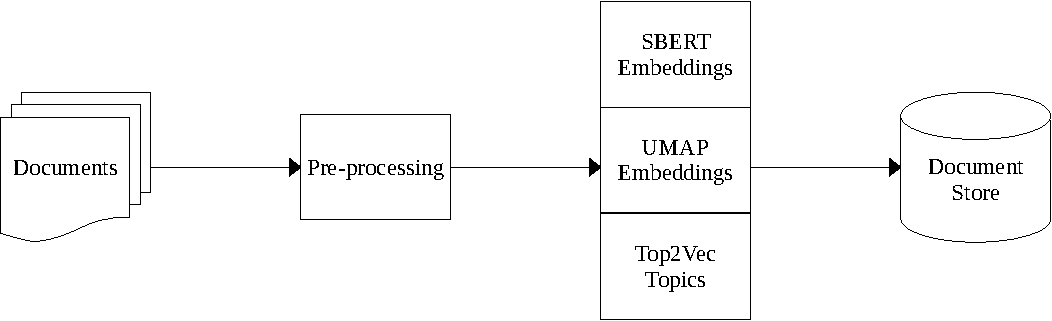
\includegraphics[scale=0.7]{./figures/indexing_pipeline}
	\caption{Indexing Pipeline}
	\label{indexing_pipeline}
\end{figure}

\subsection*{Query}
Finding meaningful information within a large amount of data is a big part of the CI task. The ability to retrieve relevant documents from a large collection of news articles through natural language queries empowers the CI analyst with an easy and intuitive interface to scan the environment.

Our system provides a search functionality based on Open Distro for Elasticsearch and its k-Nearest Neighbor (k-NN) Search module. By utilizing the k-NN module, we can leverage the SBERT embeddings by projecting the query string onto the same semantic space as the corpus and computing its k-nearest neighbors i.e. finding the k documents which embedding vectors are closest to the query embedding vector, according to some pre-defined similarity metric. Since the embedding vectors encode the semantic identity of each document, this method provides semantically relevant results for a given query. Furthermore, the k-NN module delivers a highly performant and scalable similarity search engine by leveraging Elasticsearch’s distributed architecture and by implementing Approximate Nearest Neighbors (ANN) search based on Hierarchical Navigable Small World Graphs \citep{malkov2018}. The k-NN module can also be combined with binary filters that help the user obtain focused results based on characteristics of the documents such as publication date and category. These filters are applied directly on the database, reducing the search space as a result and improving the subsequent search time.

Once again, we can think of the search functionality as a pipeline, illustrated in Figure \ref{query_pipeline}, where we feed a query string and some binary filters, and we obtain documents ordered by their relevancy to the query. We employ a Retrieve and Re-rank pipeline based on the work of \citet{nogueira2020a, kratzwald2019} composed by a "Retrieval Bi-Enconder + ANN" node that performs semantic search using Elasticsearch’s k-NN module as described above, and by a "Re-Ranker Cross-Encoder" node consisting of a BERT \citep{devlin2019} model fine-tuned on the MS MARCO dataset that receives a document and query pair as input and predicts the probability of the document being relevant. 

The pipeline works by taking advantage of the characteristics of both nodes. The Bi-Encoder together with ANN search can retrieve fairly relevant candidates, while dealing efficiently with large collection of documents. The Cross-Encoder isn't as efficient since it has to be performed independently for each document, given a query. However, since attention is performed across the query and the document, the performance is higher in the second node. Therefore, we combine both nodes by retrieving a large set of candidates from the entire collection using the Bi-Encoder, and by filtering the most relevant candidates with the Cross-Encoder.

With this pipeline we are able to provide relevant documents to the user given a query and binary filters, while ranking them according to a relevancy score. The pipeline is efficient and makes use of the SBERT embeddings and the Elasticsearch architecture. As an additional feature, we can input a document instead of a query, allowing to search for semantically similar documents within the collection.

\begin{figure}[H]
	\centering
	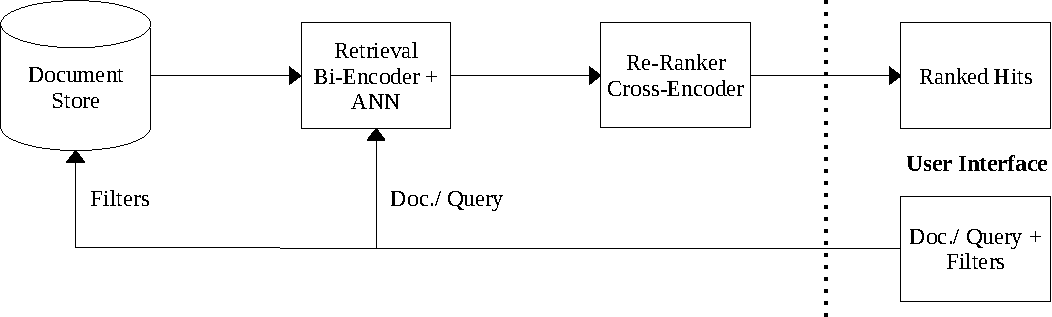
\includegraphics[scale=0.7]{./figures/query_pipeline}
	\caption{Query Pipeline}
	\label{query_pipeline}
\end{figure}

\subsection*{Visualization}
To facilitate the environment scanning task, we developed a visual interface that organizes and displays the news articles, giving the user the ability to explore the data and zoom on particular regions of the semantic space. The interface uses the UMAP \citep{mcinnes2020} algorithm to reduce the dimensionality of the original semantic space to a 2-dimensional representation that reliably preserves the original topology.

The methodology employed to produce the interface is described in Figure \ref{vis_pipeline}. It begins by taking the same inputs passed to the Query pipeline, a query and a set of filters. The common inputs create a connection between the two modules — when the user queries the database, the query text is projected onto the 2-dimensional map and the filters define which points are displayed in the map. In this way, the map can be seen as a graphical extension of the searching mechanism, where the relevant results reside in the neighborhood of the query, giving the user some insight on how the results are obtained. In addition to the common inputs, we require a relative sample size that defines the percentage of randomly chosen documents (after applying the filters) to be displayed in the map. This is necessary as interaction with the map is hindered by a large amount of data points, resulting in a slow and unresponsive experience. Notice that the sample size doesn't affect the query results, as it is always performed on the entire collection.

To produce the interactive scatter plot, the filters and sample size are used to select the documents to be displayed from the database. We compute the SBERT embedding of the query, followed by its UMAP embedding, thus being able to locate the query in the same space as the documents. An advantage of these two models is that we can efficiently produce embeddings of new text without having to re-train them, making this process quite fast. Once we have the UMAP embedding of the query, we join it with the pre-computed embeddings of the documents from the Indexing pipeline, and we produce the interactive map.

The map provides a means to explore the news articles and the different semantic cohorts present within the collection. We color-code the points with the documents' category, and when hovered, the points display their corresponding text. The map can be panned, zoomed in/out and points can be selected.

\begin{figure}[H]
	\centering
	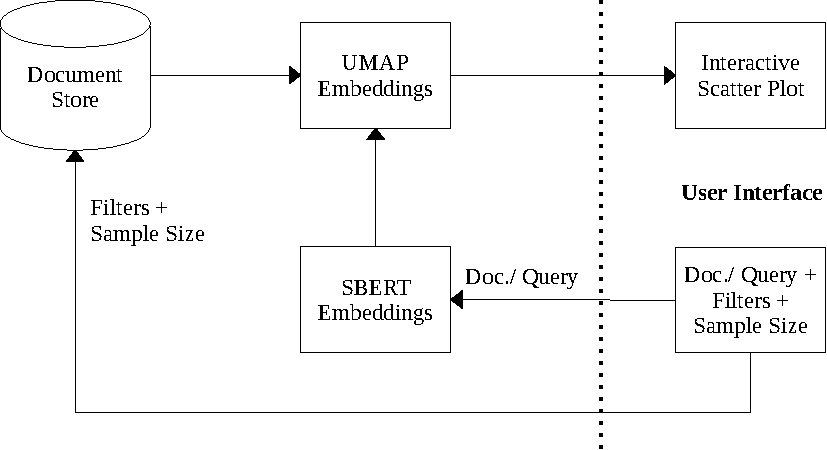
\includegraphics[scale=0.7]{./figures/vis_pipeline}
	\caption{Visualization Pipeline}
	\label{vis_pipeline}
\end{figure}

\section* {Results}
% Mention how many documents we are working with at the moment (also mention the selection procedure for this sample - data range)
Present an observation (results), then explain what happened (analysis).  Each paragraph should focus on one aspect of your results. In that same paragraph, you should interpret that result.
In other words, there should not be two distinct paragraphs, but instead one paragraph containing one result and the interpretation and analysis of this result. Here are some guiding questions for results and analysis:

When describing your results, present your data, using the guidelines below:
\begin{itemize}
	\item What happened? What did you find?
	\item Show your experimental data in a professional way. Refer to \href{https://confluence.cornell.edu/display/AGUACLARA/Grammar+Guidelines+for+Reports}{Grammar Guidelines for Reports} for details on formatting. Be sure to reference figures before they appear in your paper (see Figure \ref{Frog}). Be sure to do the same for tables (see Table \ref{Table}). For a good tool for making tables, go to \href{www.tablesgenerator.com}{tablesgenerator.com}.
\end{itemize}

\begin{figure}[H]
	\centering
	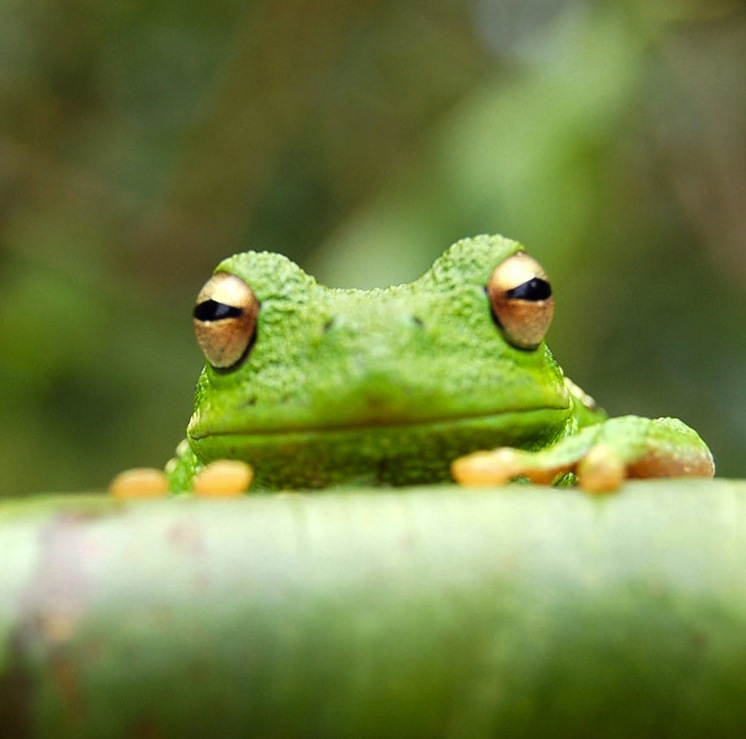
\includegraphics[scale=0.1]{./figures/frog}
	\caption{Captions go beneath figures.}
	\label{Frog}
\end{figure}

\begin{table}[H]
	\centering
	\caption{Captions go above tables.}
	\begin{tabular}{| l | c | c |}
		\hline
		Parameter          & Symbol   & Value                 \\ \hline
		Residence Time     & $\theta$ & 90 s                  \\ \hline
		Hydraulic Gradient & $G$      & 500 $\mathrm{s^{-1}}$ \\
		\hline
	\end{tabular}
	\label{Table}
\end{table}

After describing a particular result, within a paragraph, go on to connect your work to fundamental physics/chemistry/statics/fluid mechanics, or whatever field is appropriate. Analyze your results and compare with theoretical expectations; or, if you have not yet done the experiments, describe your expectations based on established knowledge. Include implications of your results. How will your results influence the design of AguaClara plants? If possible provide clear recommendations for design changes that should be adopted. Show your experimental data in a professional way using the following guidelines:
\begin{itemize}
	\item Why did you get those results/data?
	\item Did these results line up with expectations?
	\item What went wrong?
	\item If the data do not support your hypothesis, is there another hypothesis that describes your new data?
\end{itemize}

\section*{Discussion}
Study comparison with other studies. What were the limitations?

\section*{Conclusions}
Explain what you have learned and how that influences your next steps. Why does what you discovered matter to AguaClara?
Make sure that you defend your conclusions. (this is conclusions, not opinions!)

\section*{Future Work}
% Describe your plan of action for the next several weeks of research. Detail the next steps for this team. How can AguaClara use what you discovered for future projects? Your suggestions for challenges for future teams are most welcome. Should research in this area continue?
For implementing the query feature of the system, the query is embedded in the same space of the news article corpus and the distance with each SOM unit is computed. The query is then matched with the closest SOM unit and the documents allocated to that unit are retrieved. This approach is fast since there are many fewer units than documents. The unit's documents are ranked by computing the distance between them and the query. The search quality is expected to not decrease significantly as long as the Mean Quantization Error (MQE) (i.e. the mean euclidean distance each input vector to its BMU) remains low.

We plan to provide a zooming capability on the SOM U-matrix so the user can explore specific regions of the map in detail. There are two ways we have been discussing on how to implement this: one possibility would be to allow the user to select a specific unit or group of units on the map and then provide a projection of the underlying documents using either t-SNE \citep{vandermaaten2008} or UMAP \citep{mcinnes2020}; a second possibility would be to allow the user to digitally zoom in on the U-matrix, just like it is done in \citet{kaski1998}. An appealing attribute of this option is the preservation of the landmark labels, which are updated according to the zooming of the map.

There's also some discussion on how to integrate release date information on the article's representation. This would allow the documents to be organized not only according to their semantics but also according to their release date. This could also improve the query results as the users are most likely interested on current information. Another feature related to release date would be to relate documents in a time line, allowing a specific subject to be tracked through time. 

We would also like to improve the data collection pipeline since we are relying directly on NewsAPI free subscription which has some limitations already described. This would require a substantial effort since web scrapping would most likely be the necessary solution. This approach would provide us with the full article content and would allow us to collect articles as soon as they are released. Multilingual articles could also be collected and integrated into the system by using multilingual embeddings models such as \citet{conneau2019}.

Some more ideas to explore consist on: build a single or multi article summary feature, to provide a brief resume of the content of a specific article or of a specific SOM unit (collection of articles); add a news article feed based on individual user viewing history. If we plan to expand the application to multiple users, an implicit feedback collaborative filtering \citep{hu2008} approach could be used.

Some research on understanding the document embedding dimensions' would also be interesting as these usually present a correlation structure which captures the latent semantical topics of the document collection as seen in \citet{ji2019}. This would provide the user with the necessary confidence on the neural document embeddings that is lacking because of the black-box nature of these models.

\bibliographystyle{apalike}
\bibliography{bibliography}
\end{document}